\documentclass[12pt]{article}
\usepackage[utf8]{inputenc}
\usepackage{cite}  
\usepackage{setspace}
\usepackage{graphicx}
\usepackage{geometry}
\usepackage{titling} 
\usepackage{tikz-uml}
\usepackage{tikz}
\usepackage{pgfmath}
\usetikzlibrary{calc}
\usetikzlibrary{arrows.meta,shapes.geometric, positioning, shapes.multipart}
\usepackage{pgfgantt}
\usepackage{float}
\geometry{a4paper, margin=1in}
\doublespacing


\usepackage{hyperref}
\hypersetup{
	colorlinks=true,
	linkcolor=black,
	citecolor=black
}

\date{\today}

\begin{document}
	\begin{titlepage}
		\centering
		
		% College Logo
		
\includegraphics[width=0.25\textwidth]{college_logo.png}\par\vspace{1cm}
		
		% Title
		{\Huge \textbf{Software Requirements Specification}\par}
		\vspace{0.5cm}
		{\LARGE \textit{Paper Generator Web Application}\par}
		\vspace{1cm}
		
		% Authors
		{\large \textbf{Prepared By:}\par}
		\vspace{0.2cm}
		{\Large Talha and Sameer\par}
		\vspace{0.5cm}
		
		% Department
		{\large BS Information Technology\par}
		{\large Government Islamia Graduate College, Kasur\par}
		\vspace{2cm}
		
		% Horizontal line
		\rule{\linewidth}{0.5pt}\par
		\vspace{0.3cm}
		{\large \textbf{Instructor:} Faisal Hameed\par}
		\vspace{0.3cm}
		\rule{\linewidth}{0.5pt}\par
		
		\vfill
		
		% Date at the bottom
		{\large \today\par}
	\end{titlepage}
	\newpage
	\tableofcontents
	\newpage
	
	\section{Introduction}
	
	\subsection{Purpose}
	In most academic institutions, teachers spend significant time manually preparing examination materials such as quizzes, assignments, midterm exams, and final exams. This process involves gathering questions from multiple sources, ensuring appropriate coverage of topics, and adjusting difficulty levels. Such manual effort is not only time-consuming but also increases the risk of errors, inconsistency, and repetition in question selection.
	
	The Paper Generator Web Application is designed to address these challenges by automating the creation of academic assessments. The system provides a centralized question bank where teachers can store, categorize, and retrieve questions based on subject, topic, and difficulty level. It enables the generation of various types of assessments—including quizzes, assignments, midterm exams, and final exams—either randomly or through customized selection by the teacher.
	
	A key feature of this system is its ability to generate papers according to difficulty levels, such as easy, moderate, or advanced, allowing teachers to tailor exams to the required standard of evaluation. This ensures balanced assessment while promoting fairness and efficiency.
	
	The primary benefit of the Paper Generator Web Application is to enhance productivity, accuracy, and reliability in the academic evaluation process. By reducing the manual workload of teachers, the system not only saves time but also improves the quality and consistency of assessments. In the long run, it provides an adaptable solution that supports the needs of academic institutions at multiple levels of testing.
	
	\subsection{Scope}
	The Paper Generator Web Application is a web-based system designed to assist academic institutions in the creation of assessment materials, including quizzes, assignments, midterm examinations, final examinations, and other classroom tests. The system offers a centralized question bank where teachers can create, categorize, and retrieve questions based on subject, topic, and difficulty level.
	
	The application also enables teachers to upload course materials—such as PDFs, Word documents, and digital notes—which the system analyzes to automatically generate relevant questions. This ensures that the assessments produced are accurately aligned with the specific course content.
	
	Teachers can generate examination papers either randomly or through manual selection of questions. The system supports difficulty-based paper generation (easy, moderate, advanced), ensures balanced distribution of questions, minimizes repetition, and allows exporting the final paper in printable formats such as PDF or Word.
	
	
	This project is limited to the generation and management of assessment papers. It does not include automated grading, plagiarism detection, student management, result processing, or online examination delivery. Its primary objective is to reduce manual effort, enhance accuracy, and improve the efficiency of examination preparation for teachers and academic administrators.
	
	\subsection{Overview}
	The Paper Generator Web Application is a web-based system designed to automate the creation of academic assessments. It provides an efficient and reliable alternative to the traditional manual method of preparing quizzes, assignments, midterm exams, and final examinations. The system is intended primarily for teachers and academic staff involved in paper preparation across various educational levels.
	
	The application allows users to upload course materials—such as PDFs, textbooks, and digital notes—from which the system can automatically generate relevant questions. A centralized question bank is also provided for the manual creation, categorization, and storage of questions.
	
	The system supports the generation of examination papers based on difficulty levels (easy, moderate, advanced) and offers export options in both PDF and Word formats to facilitate distribution and printing. As a web-based platform backed by a secure database, the system ensures scalability, accessibility, and long-term maintainability for academic institutions.
	
	\subsection{Definitions, Acronyms, and Abbreviations}
	
	\begin{description}
		\item[Admin] The system administrator who manages user accounts, maintains the question bank, and oversees overall system operations.
		
		\item[Automatic Paper Generator] The proposed web application that automates the creation of quizzes, assignments, midterm, and final examination papers.
		
		\item[Authentication] The process of verifying the identity of a user before granting access to the system.
		
		\item[Database] A structured collection of data used to store and retrieve questions, user information, and exam templates.
		
		\item[Exam Template] A predefined structure or format that specifies the distribution of questions in an examination paper (e.g., number of MCQs, short questions, long questions).
		
		\item[PDF (Portable Document Format)] A digital file format used for exporting and distributing generated exam papers.
		
		\item[Question Bank] A repository within the system where questions are stored, categorized by subject, topic, difficulty level, and type.
		
		\item[SRS (Software Requirements Specification)] The document that specifies the functional and non-functional requirements of the system.
		
		\item[UI (User Interface)] The part of the application that allows interaction between the user and the system.
	\end{description}
	
	
	\section{Overall Description}
	
	\subsection{Product Perspective}
	The Paper Generator Web Application is a web-based standalone system that automates the creation of quizzes, assignments, midterms, and final exams, replacing the manual paper preparation process.
	
	Teachers can upload course materials (PDFs, Word documents, textbooks) or use a centralized question bank to generate questions automatically, organized by subject, topic, and difficulty.
	
	The system allows paper generation by difficulty level — Easy, Moderate, or Advanced — and supports exporting papers in PDF or Word format for easy printing or digital use.
	
	It runs as a web application accessible through modern browsers and uses a secure database, making it fully standalone, scalable, and reliable for academic institutions.

	\subsection{Product Functions}
	\begin{itemize}
		\item \textbf{Course Material Management:}
		The system allows teachers to upload course materials such as PDFs, Word documents, and digital textbooks. It automatically analyzes the uploaded files and extracts relevant questions, which are then stored in the centralized question bankk.
		\item \textbf{Question Bank Management:}Teachers can manually create, edit, categorize, and store questions in the question bank. Questions can be organized and retrieved based on subject, topic, question type, and difficulty level to ensure structured content management.
		\item \textbf{Paper Generation:} The system can generate quizzes, assignments, midterm exams, and final examinations using either uploaded course material or existing question bank entries. Teachers can select the desired difficulty level (easy, moderate, or advanced), and the system ensures balanced distribution and avoids repetition of questions.
		\item \textbf{Export and Printing:} Generated papers can be exported in PDF or Word format. Before finalizing, teachers can preview the paper and make necessary adjustments, such as editing questions, rearranging order, or modifying marks distribution.
		\item \textbf{User Management (Optional):} The system may include user account creation and authentication for teachers. This allows secure access to uploaded materials, stored questions, and previously generated papers.
	\end{itemize}
	
	\subsection{User Classes and Characteristics}
	\begin{itemize}
		\item \textbf{Teachers / Professors:} Primary users responsible for uploading course material, managing the question bank, and generating assessments. They are expected to have basic computer skills and familiarity with web applications.
		\item \textbf{Administrators (Optional):} Responsible for managing user accounts and maintaining the system. They ensure proper access control and data integrity.
		\item \textbf{System Access Requirements:} All users require a modern web browser and internet connection. Teachers need access to course materials in standard formats (PDF, Word).
	\end{itemize}
	
	\subsection{Operating Environment}
	The Paper Generator Web Application is a web-based system accessible through modern browsers such as Chrome, Edge, and Firefox. It runs on standard desktop or laptop computers and does not require specialized hardware.
	
	The system uses a secure server-side database to store course materials, questions, and generated papers. Internet connectivity is required for full functionality, including uploading materials and exporting papers.
	
	The application is designed to be scalable and platform-independent, allowing easy deployment in academic institutions of various sizes. It supports standard file formats (PDF, Word) for input and output.
	
	\subsection{Design and Implementation Constraints}
	\begin{itemize}
		\item \textbf{Web-Based Platform:} The system must run as a web application compatible with modern browsers. It cannot rely on desktop-only software.
		\item \textbf{File Format Support:} Uploaded course materials must be in standard formats (PDF, Word) to ensure proper question extraction.
		\item \textbf{Internet Requirement:} A stable internet connection is necessary for uploading materials, generating papers, and exporting files.
		\item \textbf{Database Dependency:} The system relies on a secure server-side database for storing course materials, questions, and generated papers.
		\item \textbf{Scalability Limitations:} Performance may depend on server capacity and the number of concurrent users, especially in large institutions.
	\end{itemize}
	
	\subsection{Assumptions and Dependencies}
	\begin{itemize}
		\item \textbf{Teacher-Provided Materials:} The system assumes that teachers provide course materials in standard formats (PDF, Word) for question extraction. Improperly formatted files may affect functionality.
		\item \textbf{Internet Connectivity:} A stable internet connection is required for uploading materials, generating papers, and exporting files.
		\item \textbf{Browser Compatibility:} Users are expected to access the system through modern web browsers such as Chrome, Edge, or Firefox.
		\item \textbf{Server and Database Availability:} The system depends on a secure, functioning server and database to store course materials, questions, and generated papers. Any server downtime may affect operations.
		\item \textbf{User Competency:} Teachers using the system are assumed to have basic computer skills and familiarity with web applications.
	\end{itemize}
	
	
	\section{System Features}
	
	
	\subsection{Functional Requirements}
	
	\subsubsection{User Authentication}
	\begin{itemize}
		\item Teachers must register with name, email, and password.
		\item Teachers log in using valid credentials.
		\item The system supports password reset through email verification.
	\end{itemize}
	
	\subsubsection{Course Material Management}
	\begin{itemize}
		\item Teachers can upload course materials in PDF or Word format.
		\item Uploaded files are processed to extract questions automatically.
		\item The system validates file types before upload.
	\end{itemize}
	
	\subsubsection{Question Bank Management}
	\begin{itemize}
		\item Teachers can add, edit, delete, and categorize questions.
		\item Questions are organized by subject, topic, and difficulty.
		\item The system prevents duplication in the database.
		\item Search and filter options are available by keyword, topic, or difficulty.
	\end{itemize}
	
	\subsubsection{Paper Generation}
	\begin{itemize}
		\item Teachers can create quizzes, assignments, midterms, and finals.
		\item Papers can be generated randomly or through manual selection.
		\item Teachers can set difficulty levels (Easy, Moderate, Hard).
		\item Generated papers include metadata such as subject, exam type, and total marks.
	\end{itemize}
	
	\subsubsection{Export and Printing}
	\begin{itemize}
		\item Generated papers can be exported in PDF or Word format.
		\item Teachers can preview and edit papers before finalizing.
		\item The system supports printing and downloading exam papers.
	\end{itemize}
	
	\subsubsection{Notifications and Feedback}
	\begin{itemize}
		\item System provides success/error notifications for uploads, edits, and paper generation.
		\item Teachers receive confirmation when an exam paper is generated successfully.
	\end{itemize}
	
	\subsubsection{Admin Functions}
	\begin{itemize}
		\item Admins can manage teacher accounts.
		\item Admins can monitor system usage and database growth.
		\item Admins have access to audit logs for troubleshooting.
	\end{itemize}
	
	
	
	\subsection{Non-Functional Requirements}
	
	\subsubsection{Performance}
	\begin{itemize}
		\item The system must generate exam papers within 3--5 seconds, even when processing large question banks.
		\item Response time for user interactions (e.g., searching questions, filtering topics) should not exceed 2 seconds.
		\item The application should be optimized to handle up to 10,000+ stored questions without significant delay.
		\item Performance testing must be conducted to ensure acceptable speed under normal and peak loads.
	\end{itemize}
	
	\subsubsection{Usability}
	\begin{itemize}
		\item The user interface must be simple, consistent, and intuitive, allowing teachers to navigate without prior technical knowledge.
		\item Common tasks (e.g., uploading materials, generating papers) should be achievable in no more than 3--4 clicks.
		\item The system should provide tooltips, error messages, and help guides to assist users when needed.
		\item Usability testing with representative users (teachers) must be performed to ensure ease of use.
	\end{itemize}
	
	\subsubsection{Reliability}
	\begin{itemize}
		\item The system must generate exam papers accurately without duplication or missing content.
		\item It should ensure proper and secure storage of course materials and the question bank.
		\item In case of failures such as network interruptions or system crashes, the system must recover without data loss.
		\item Regular backups and error-handling mechanisms should be in place to guarantee dependable operation.
	\end{itemize}
	
	\subsubsection{Scalability}
	\begin{itemize}
		\item The system should support multiple concurrent users without performance degradation.
		\item It must efficiently handle an expanding question bank as the database grows over time.
		\item The architecture should allow easy scaling of resources, such as storage and processing power, to meet future demands.
		\item The system should maintain consistent response times as the number of users and stored questions increases.
	\end{itemize}
	
	\subsubsection{Security}
	\begin{itemize}
		\item The system must protect course materials, question banks, and generated papers from unauthorized access.
		\item User authentication should be required before accessing the system.
		\item Role-based access control must be implemented to differentiate permissions between admins and teachers.
		\item All sensitive data should be encrypted during storage and transmission.
		\item Regular security audits and updates must be performed to safeguard against vulnerabilities.
	\end{itemize}
	
	\subsubsection{Portability}
	\begin{itemize}
		\item The system should be compatible with all major modern web browsers, including Chrome, Firefox, Edge, and Safari.
		\item It must run smoothly on different operating systems such as Windows, macOS, and Linux.
		\item The application should be accessible on various devices, including desktops, laptops, tablets, and smartphones.
		\item The design should follow responsive web standards to ensure a consistent user experience across platforms.
	\end{itemize}
	
	\subsubsection{Maintainability}
	\begin{itemize}
		\item Maintenance is the process of keeping the system in proper working condition after deployment.
		\item It includes fixing bugs, applying updates, and improving features to ensure smooth operation.
		\item Regular maintenance prevents major failures and extends the system’s usable life.
		\item Maintenance activities include corrective, adaptive, perfective, and preventive actions.
		\item Effective maintenance ensures the system continues to meet user needs and adapts to new requirements.
	\end{itemize}
	
	
	\section{Technology Stack}
	
	\subsection{Front End}
	\begin{itemize}
		\item The front end will be developed using \textbf{React.js} to build a dynamic and responsive user interface.
		\item \textbf{HTML5} and \textbf{CSS3} will be used for structuring and styling the application.
		\item \textbf{JavaScript (ES6+)} features will enhance interactivity and improve performance.
	\end{itemize}
	
	\subsection{Back End}
	\begin{itemize}
		\item The back end will be powered by \textbf{Node.js} for handling server-side logic efficiently.
		\item \textbf{Express.js} will be used as the framework to manage APIs and streamline backend development.
		\item \textbf{RESTful APIs} will connect the client-side with the server-side securely.
	\end{itemize}
	
	\subsection{Database}
	\begin{itemize}
		\item \textbf{MongoDB} will be used as the NoSQL database to store questions, templates, and user information.
		\item Its document-oriented model supports scalability and flexibility for the growing question bank.
		\item Indexing and replication will ensure efficient data retrieval and reliability.
	\end{itemize}
	
	\subsection{Development Tools}
	\begin{itemize}
		\item \textbf{Visual Studio Code (VS Code)} will serve as the primary IDE for development.
		\item \textbf{Git and GitHub} will be used for version control and collaborative development.
		\item \textbf{Postman} will assist in testing APIs, while browser developer tools will support debugging and optimization.
	\end{itemize}
	\newpage
	\section{System Models}
	\subsection{Use Case Diagram}
	
	The following use case diagram illustrates the main interactions between the actors (Teacher and Admin) and the Paper Generator Web Application:
	
	\begin{center}
		\begin{tikzpicture}
			
			% System boundary
			\begin{umlsystem}[x=6, y=0]{Paper Generator Web Application}
				\umlusecase[y=0]{User Authentication}
				\umlusecase[y=-2]{Course Material Management}
				\umlusecase[y=-4]{Question Bank Management}
				\umlusecase[y=-6]{Paper Generation}
				\umlusecase[y=-8]{Export \& Printing}
				\umlusecase[y=-10]{Notifications \& Feedback}
				\umlusecase[y=-12]{Admin Functions}
			\end{umlsystem}
			
			% Actors
			\umlactor[x=0, y=-3]{Teacher}
			\umlactor[x=12, y=-6]{Admin}
			
			% Associations Teacher ↔ Use cases
			\umlassoc{Teacher}{usecase-1} % Authentication
			\umlassoc{Teacher}{usecase-2} % Course Material Management
			\umlassoc{Teacher}{usecase-3} % Question Bank Management
			\umlassoc{Teacher}{usecase-4} % Paper Generation
			\umlassoc{Teacher}{usecase-5} % Export & Printing
			\umlassoc{Teacher}{usecase-6} % Notifications & Feedback
			
			% Associations Admin ↔ Use cases
			\umlassoc{Admin}{usecase-1} % Authentication
			\umlassoc{Admin}{usecase-7} % Admin Functions
			
			% Include/Extend relationships
			\umlinclude{usecase-4}{usecase-3} % Paper Generation includes Question Bank
			\umlinclude{usecase-4}{usecase-2} % Paper Generation includes Course Material
			\umlextend{usecase-5}{usecase-4}  % Export extends Paper Generation
			
		\end{tikzpicture}
	\end{center}
	\newpage
	\subsection{Use Case Diagram: Paper Generation}
	
	The following diagram shows the detailed use case for the Paper Generation feature:
	
	\begin{center}
		\begin{tikzpicture}
			
			% System boundary
			\begin{umlsystem}[x=6, y=0]{Paper Generator}
				\umlusecase[y=0]{Paper Generation}            % usecase-1
				\umlusecase[y=-2.1]{Question Bank Management}  % usecase-2
				\umlusecase[y=-4.2]{Course Material Management}  % usecase-3
				\umlusecase[y=-6]{Export \& Printing}        % usecase-4
			\end{umlsystem}
			
			% Actor
			\umlactor[x=-2, y=-2]{Teacher}
			
			% --- Associations from Teacher to all Use Cases ---
			\umlassoc[anchor1=east, anchor2=west]{Teacher}{usecase-1}
			\umlassoc[anchor1=east, anchor2=west]{Teacher}{usecase-2}
			\umlassoc[anchor1=east, anchor2=west]{Teacher}{usecase-3}
			\umlassoc[anchor1=east, anchor2=west]{Teacher}{usecase-4}
			

		\end{tikzpicture}
	\end{center}
	
	
	\subsubsection*{Use Case Description: Paper Generation}
	
	\textbf{Actors:} Teacher (Primary Actor)
	
	\textbf{Goal:} To generate quizzes, assignments, midterms, and final examination papers by using questions from the Question Bank or uploaded Course Materials.
	
	\textbf{Preconditions:}
	\begin{itemize}
		\item The Teacher is authenticated and logged into the system.
		\item Relevant questions exist in the Question Bank and/or Course Materials have been uploaded.
	\end{itemize}
	
	\textbf{Postconditions:}
	\begin{itemize}
		\item A draft paper is generated based on the Teacher’s selected parameters (exam type, difficulty, number of questions).
		\item The Teacher may choose to export the finalized paper for distribution.
	\end{itemize}
	
	\textbf{Main Flow:}
	\begin{enumerate}
		\item The Teacher selects the \textit{Paper Generation} option.
		\item The system prompts the Teacher to provide exam details such as type (quiz, assignment, midterm, final), subject, and difficulty level.
		\item The system retrieves questions from the \textbf{Question Bank} and/or processes uploaded \textbf{Course Material}.
		\item The system compiles the exam paper according to the selected parameters.
		\item The Teacher reviews the draft paper and finalizes it.
		\item Optionally, the Teacher uses the \textit{Export \& Printing} feature to save or distribute the paper in PDF/Word format.
	\end{enumerate}
	
	\textbf{Alternative Flows:}
	\begin{itemize}
		\item If there are insufficient questions in the Question Bank or Course Material, the system alerts the Teacher to add or upload more questions.
		\item If the Teacher cancels the process, no paper is generated.
	\end{itemize}
	
	\textbf{Extensions:}
	\begin{itemize}
		\item \textbf{Export \& Printing} is modeled as an \texttt{<<extend>>} use case, providing optional functionality to produce distribution-ready documents.
	\end{itemize}
	
	\textbf{Remarks:}  
	This use case is the central functionality of the Paper Generator Web Application. It includes both \textit{Question Bank Management} and \textit{Course Material Management} through \texttt{<<include>>} relationships, ensuring that paper generation is always based on valid and organized content.
	\newpage
	\subsection{Use Case Diagram: Question Bank Management}
	
	The following diagram shows the detailed use case for managing the Question Bank:
	
	\begin{center}
		\begin{tikzpicture}
			
			% System boundary
			\begin{umlsystem}[x=6, y=0]{Question Bank Management}
				\umlusecase[y=0]{Add Questions}
				\umlusecase[y=-2.3]{Edit Questions}
				\umlusecase[y=-3.8]{Delete Questions}
				\umlusecase[y=-7.5]{Categorize Questions}
				\umlusecase[y=-5.9]{Search \& Filter}
			\end{umlsystem}
			
			% Actor
			\umlactor[x=0, y=-3]{Teacher}
			
			% Associations Teacher ↔ Use cases
			\umlassoc{Teacher}{usecase-1}
			\umlassoc{Teacher}{usecase-2}
			\umlassoc{Teacher}{usecase-3}
			\umlassoc{Teacher}{usecase-4}
			\umlassoc{Teacher}{usecase-5}
			
		\end{tikzpicture}
	\end{center}
	
	\subsubsection*{Use Case Description: Question Bank Management}
	
	\textbf{Actors:} Teacher (Primary Actor)
	
	\textbf{Goal:}  
	To maintain a centralized repository of questions by adding, editing, deleting, categorizing, and retrieving them efficiently.
	
	\textbf{Preconditions:}
	\begin{itemize}
		\item The Teacher is logged into the system.
		\item The Teacher has the necessary permissions to manage questions.
	\end{itemize}
	
	\textbf{Postconditions:}
	\begin{itemize}
		\item The Question Bank is updated according to the Teacher’s actions.
		\item All questions are stored with relevant metadata such as subject, topic, type, and difficulty level.
	\end{itemize}
	
	\textbf{Main Flow:}
	\begin{enumerate}
		\item The Teacher accesses the \textit{Question Bank Management} feature from the system.
		\item The Teacher may perform the following actions:
		\begin{itemize}
			\item Add new questions manually or import them from uploaded material.
			\item Edit existing questions to correct or update their content.
			\item Delete questions that are outdated or no longer valid.
			\item Categorize questions by subject, topic, type (MCQ, short, long), and difficulty (Easy, Moderate, Hard).
			\item Search and filter questions using keywords, categories, or difficulty level.
		\end{itemize}
		\item The system validates all changes and updates the Question Bank accordingly.
	\end{enumerate}
	
	\textbf{Alternative Flows:}
	\begin{itemize}
		\item If a duplicate question is detected, the system warns the Teacher and prevents duplication.
		\item If the Teacher attempts to delete a question linked to an existing paper, the system requests confirmation before removal.
	\end{itemize}
	
	\textbf{Remarks:}  
	This use case ensures that the Question Bank remains accurate, organized, and scalable. It plays a crucial role in supporting the \textit{Paper Generation} process by providing a reliable set of categorized and validated questions.
	\newpage
	\subsection{Use Case Diagram: Course Material Management}
	
	The following diagram shows the detailed use case for the Course Material Management feature:
	
	\begin{center}
		\begin{tikzpicture}
			
			% System boundary
			\begin{umlsystem}[x=6, y=0]{Course Material Management}
				\umlusecase[y=0]{Course Material Upload}
				\umlusecase[y=-2.3]{File Validation}
				\umlusecase[y=-4]{Question Extraction}
				\umlusecase[y=-6.3]{Store in Question Bank}
			\end{umlsystem}
			
			% Actor
			\umlactor[x=0, y=-3]{Teacher}
			
			% Associations
			\umlassoc{Teacher}{usecase-1}
			\umlassoc{Teacher}{usecase-2}
			\umlassoc{Teacher}{usecase-3}
			\umlassoc[anchor1=east, anchor2=west]{Teacher}{usecase-4} % Teacher → Course Material Upload
			
			
		\end{tikzpicture}
	\end{center}
	
	\subsubsection*{Use Case Description: Course Material Management}
	
	\textbf{Actor:} Teacher (Primary Actor)
	
	\textbf{Goal:}  
	To upload course materials (PDFs, Word documents, or textbooks), validate them, extract questions, and store them in the Question Bank for later use.
	
	\textbf{Preconditions:}
	\begin{itemize}
		\item The Teacher is logged into the system.
		\item The Teacher has access to digital course material in supported formats (PDF, Word).
	\end{itemize}
	
	\textbf{Postconditions:}
	\begin{itemize}
		\item Course material is successfully uploaded and validated.
		\item Extracted questions are stored in the Question Bank with appropriate metadata.
	\end{itemize}
	
	\textbf{Main Flow:}
	\begin{enumerate}
		\item The Teacher selects the option to upload course material.
		\item The system performs \textit{File Validation} (format and file size checks).
		\item If valid, the system extracts questions from the material.
		\item Extracted questions are automatically categorized and stored in the Question Bank.
	\end{enumerate}
	
	\textbf{Alternative Flows:}
	\begin{itemize}
		\item If the uploaded file is in an unsupported format, the system shows an error message.
		\item If extraction fails due to poor formatting, the system notifies the Teacher and logs the issue.
	\end{itemize}
	
	\textbf{Remarks:}  
	This use case ensures that teachers can directly integrate their course materials into the system. By extracting and storing questions automatically, it reduces manual workload and keeps the Question Bank updated with relevant academic content.
	
	
	\newpage
\subsection{Sequence Diagram: Paper Generation}

The following refined sequence diagram illustrates the interaction between
the Teacher and the Paper Generator Web Application during the paper creation
and export process.

\begin{center}
	\resizebox{0.95\textwidth}{!}{
		\begin{tikzpicture}
			\begin{umlseqdiag}
				
				% Participants
				\umlactor[class=Teacher, fill=yellow!20]{teacher}
				\umlobject[class=System, fill=blue!10]{system}
				\umlobject[class=Question Bank, fill=green!10]{qbank}
				\umlobject[class=Paper Generator, fill=orange!10]{pgenerator}
				\umlobject[class=Database, fill=purple!10]{database}
				\umlobject[class=Export Module, fill=cyan!10]{export}
				
				% Login
				\begin{umlcall}[op=login(), return=success, type=synchron]{teacher}{system}
				\end{umlcall}
				
				% Teacher selects course
				\begin{umlcall}[op=selectCourse(), return=courseDetails, type=synchron]{teacher}{system}
				\end{umlcall}
				
				% System asks Paper Generator to prepare paper
				\begin{umlcall}[op=initiatePaperGeneration(), type=synchron]{system}{pgenerator}
				\end{umlcall}
				
				% Paper Generator generates the final paper
				\begin{umlcall}[op=generatePaper(), type=synchron]{pgenerator}{pgenerator}
				\end{umlcall}
				
				% Store paper
				\begin{umlcall}[op=storePaper(), return=stored, type=synchron]{pgenerator}{database}
				\end{umlcall}
				
				% Teacher requests export (to System)
				\begin{umlcall}[op=requestExport(), type=synchron]{teacher}{system}
				\end{umlcall}
				
				% System sends export request to Export Module
				\begin{umlcall}[op=exportPDF(), type=synchron]{system}{export}
				\end{umlcall}
				
				% Export Module returns the generated PDF to System
				\begin{umlcreatecall}[class=GeneratedPDF]{system}{teacher}
				\end{umlcreatecall}
				
			\end{umlseqdiag}
		\end{tikzpicture}
	}
\end{center}
\subsection*{Description}

This sequence diagram illustrates the paper generation workflow:
\begin{itemize}
	\item \textbf{Authentication}: Teacher logs into the System
	\item \textbf{Initialization}: Teacher selects course and initiates paper generation
	\item \textbf{Paper Creation}: Paper Generator composes the exam paper and stores it in the Database
	\item \textbf{Export}: Teacher requests and receives the final paper as PDF via the Export Module
\end{itemize}

\newpage

\subsection{Sequence Diagram: Question Bank Management}

The following sequence diagram illustrates how a Teacher interacts with the system to manage the Question Bank — including adding, editing, and retrieving questions.

\begin{center}
	\resizebox{\textwidth}{!}{%
		\begin{tikzpicture}
			\begin{umlseqdiag}
				
				% Participants
				\umlactor[class=Teacher, fill=yellow!20]{teacher}
				\umlobject[class=System, fill=blue!10]{system}
				\umlobject[class=Question Bank, fill=green!10]{qbank}
				\umlobject[class=Database, fill=purple!10]{database}
				
				% Messages with manual padding
				\begin{umlcall}[op={Login()}, return={Success}, type=synchron, dt=8]{teacher}{system}
				\end{umlcall}
				
				\begin{umlcall}[op={OpenQuestionBank()}, return={InterfaceLoaded}, type=synchron, dt=8]{teacher}{system}
				\end{umlcall}
				
				\begin{umlcall}[op={FetchQuestions()}, return={QuestionList}, type=synchron, dt=8]{system}{database}
				\end{umlcall}
				
				%\begin{umlcall}[op={DisplayQuestions()}, type=synchron, dt=8]{system}{qbank}
				%\end{umlcall}
				
				\begin{umlcall}[op={AddQuestion()}, return={Success}, type=synchron, dt=8]{teacher}{qbank}
				\end{umlcall}
				
				\begin{umlcall}[op={StoreQuestion()}, return={Stored}, type=synchron, dt=8]{qbank}{database}
				\end{umlcall}
				
				\begin{umlcall}[op={EditQuestion()}, return={Updated}, type=synchron, dt=8]{teacher}{qbank}
				\end{umlcall}
				
				\begin{umlcall}[op={DeleteQuestion()}, return={Removed}, type=synchron, dt=8]{teacher}{qbank}
				\end{umlcall}
				
			\end{umlseqdiag}
		\end{tikzpicture}
	}
\end{center}

%\noindent\textbf{Description:}  
%\noindent\textbf{Description:}  
\subsection*{Description}
This sequence diagram illustrates the question bank management workflow:
\begin{itemize}
	\item \textbf{Authentication}: Teacher logs into the System
	\item \textbf{Access}: Teacher opens the Question Bank interface
	\item \textbf{Retrieval}: System fetches existing questions from Database
	\item \textbf{Management}: Teacher performs Add, Edit, and Delete operations on questions
	\item \textbf{Persistence}: All changes are stored in the Database
\end{itemize}


\subsection{Sequence Diagram: Course Material Management}

The following sequence diagram illustrates how a teacher uploads and manages course materials within the Paper Generator Web Application.

\begin{center}
	\resizebox{\textwidth}{!}{%
		\begin{tikzpicture}
			\begin{umlseqdiag}
				
				% Participants
				\umlactor[class=Teacher, fill=yellow!20]{teacher}
				\umlobject[class=System, fill=blue!10]{system}
				\umlobject[class=File Processor, fill=orange!10]{fileproc}
				\umlobject[class=Question Extractor, fill=green!10]{qextract}
				\umlobject[class=Database, fill=purple!10]{database}
				
				% Message sequence
				\begin{umlcall}[op=Login(), return=Success, type=synchron]{teacher}{system}
				\end{umlcall}
				
				\begin{umlcall}[op=UploadMaterial(File.pdf), return=Received, type=synchron]{teacher}{system}
				\end{umlcall}
				
				\begin{umlcall}[op=ValidateFile(), return=Valid, type=synchron]{system}{fileproc}
				\end{umlcall}
				
				\begin{umlcall}[op=ExtractQuestions(), return=QuestionSet, type=synchron]{fileproc}{qextract}
				\end{umlcall}
				
				\begin{umlcall}[op=StoreExtractedQuestions(), return=Stored, type=synchron]{qextract}{database}
				\end{umlcall}
				
				\begin{umlcall}[op=NotifyUploadSuccess(), type=synchron]{system}{teacher}
				\end{umlcall}
				
			\end{umlseqdiag}
		\end{tikzpicture}
	}
\end{center}

\noindent\textbf{Description:}  
This sequence diagram illustrates the course material upload workflow:
\begin{itemize}
	\item \textbf{Authentication}: Teacher logs into the System
	\item \textbf{Upload}: Teacher submits course material file
	\item \textbf{Processing}: System validates file and extracts questions
	\item \textbf{Storage}: Extracted questions are saved to Database
	\item \textbf{Confirmation}: Teacher receives upload success notification
\end{itemize}

\newpage

\subsection{System State Diagram: Paper Generator Application}

The following state diagram presents the main flow of the Paper Generator Web Application.

\begin{center}
	\resizebox{0.98\textwidth}{!}{ % Auto-fit to page width
		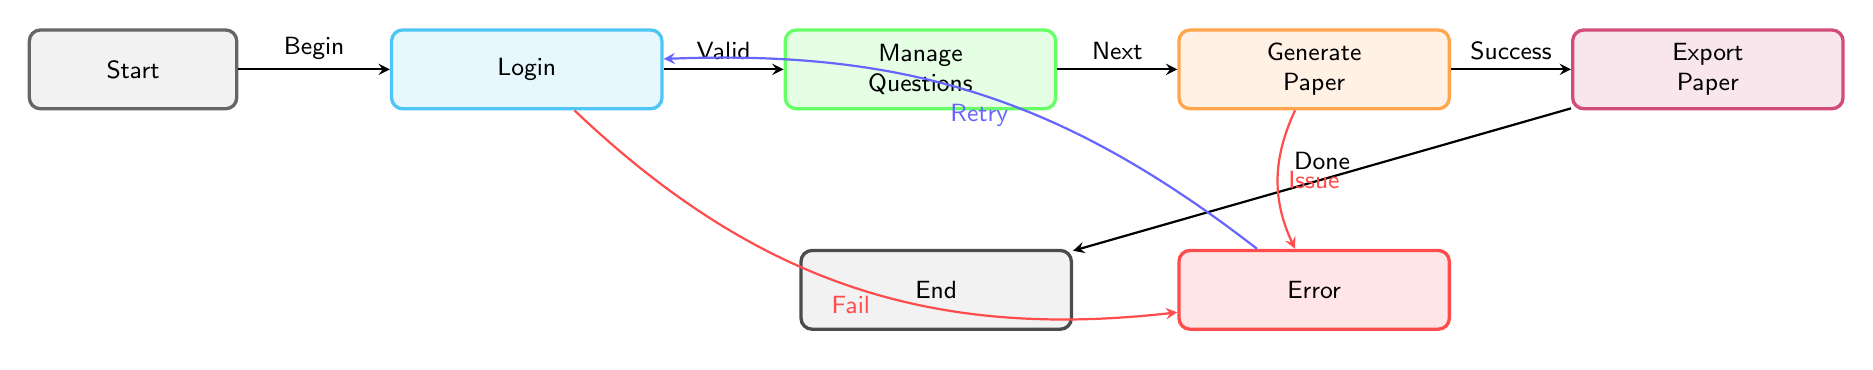
\begin{tikzpicture}[->, >=stealth, node distance=5cm,
			every node/.style={font=\sffamily\small},
			state/.style={rectangle, rounded corners, draw=blue!60, very thick,
				text width=3.2cm, align=center, fill=blue!5, minimum height=1cm}]
			
			% States
			\node[state, fill=gray!10, draw=black!60, text width=2.4cm] (start) {Start};
			\node[state, right of=start, fill=cyan!10, draw=cyan!70] (login) {Login};
			\node[state, right of=login, fill=green!10, draw=green!60] (manage) {Manage\\Questions};
			\node[state, right of=manage, fill=orange!10, draw=orange!70] (generate) {Generate\\Paper};
			\node[state, right of=generate, fill=purple!10, draw=purple!70] (export) {Export\\Paper};
			\node[state, below of=generate, fill=red!10, draw=red!70, node distance=2.8cm] (error) {Error};
			\node[state, left of=error, fill=gray!10, draw=black!70, node distance=4.8cm] (end) {End};
			
			% Transitions
			\path (start) edge[thick] node[above]{Begin} (login)
			(login) edge[thick] node[above]{Valid} (manage)
			(manage) edge[thick] node[above]{Next} (generate)
			(generate) edge[thick] node[above]{Success} (export)
			(export) edge[thick] node[above]{Done} (end)
			(login) edge[bend right=25, thick, red!70] node[below]{Fail} (error)
			(generate) edge[bend right=25, thick, red!70] node[right]{Issue} (error)
			(error) edge[bend right=20, thick, blue!60] node[below]{Retry} (login);
			
		\end{tikzpicture}
	}
\end{center}

\subsection{State Diagram: Paper Generation Process}

The following state diagram illustrates the workflow of the Paper Generation feature, showing the transitions between different system states.

\begin{center}
	\resizebox{0.98\textwidth}{!}{ % slightly larger than before
		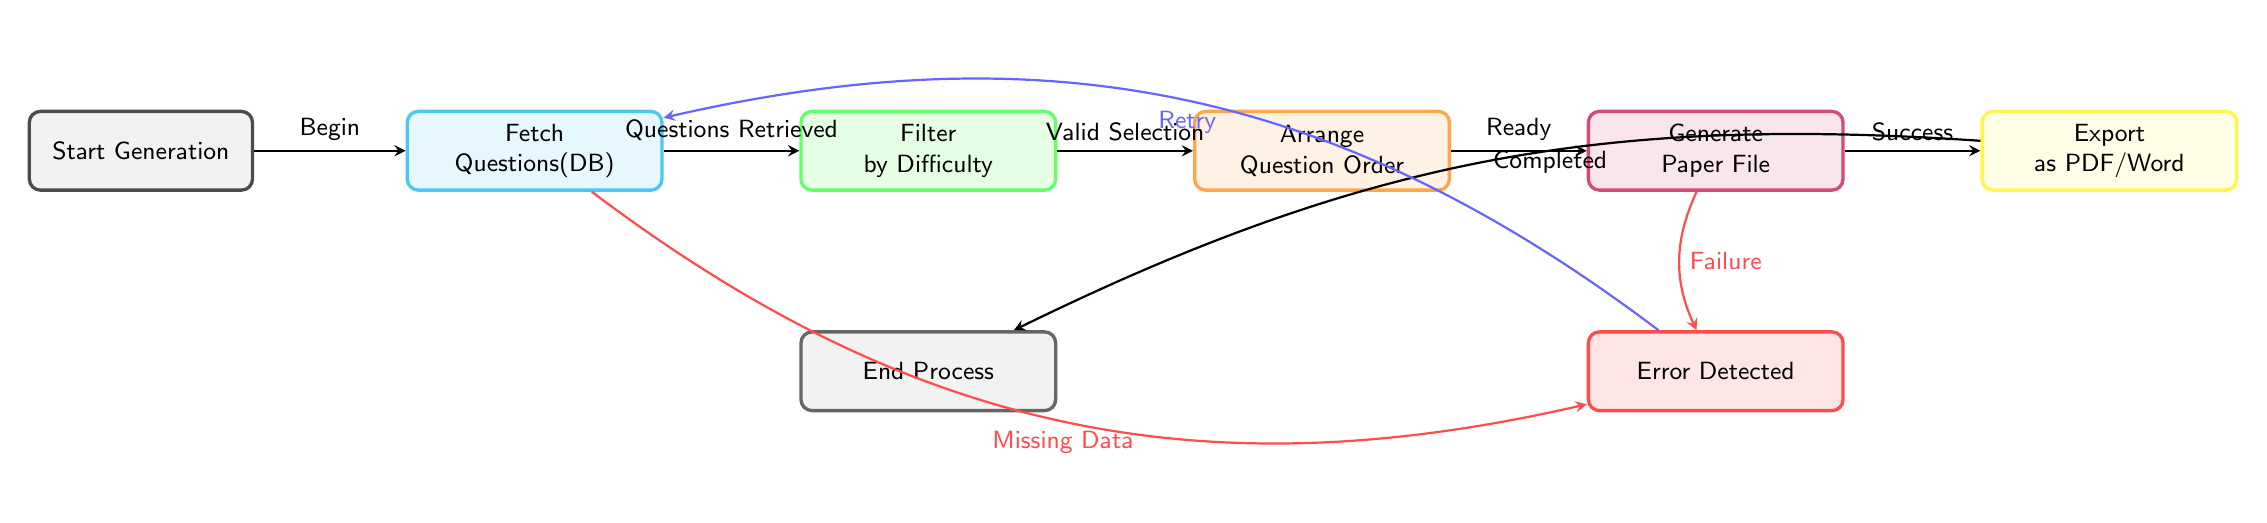
\begin{tikzpicture}[->, >=stealth, node distance=5cm,
			every node/.style={font=\sffamily\small},
			state/.style={rectangle, rounded corners, draw=blue!60, very thick,
				text width=3cm, align=center, fill=blue!5, minimum height=1cm}]
			
			% States
			\node[state, fill=gray!10, draw=black!70, text width=2.6cm] (start) {Start Generation};
			\node[state, right of=start, fill=cyan!10, draw=cyan!70] (fetch) {Fetch\\Questions(DB)};
			\node[state, right of=fetch, fill=green!10, draw=green!60] (filter) {Filter\\by Difficulty};
			\node[state, right of=filter, fill=orange!10, draw=orange!70] (arrange) {Arrange\\Question Order};
			\node[state, right of=arrange, fill=purple!10, draw=purple!70] (generate) {Generate\\Paper File};
			\node[state, right of=generate, fill=yellow!10, draw=yellow!70] (export) {Export\\as PDF/Word};
			\node[state, below of=generate, fill=red!10, draw=red!70, node distance=2.8cm] (error) {Error Detected};
			\node[state, below of=filter, fill=gray!10, draw=black!60, node distance=2.8cm] (end) {End Process};
			
			% Transitions
			\path (start) edge[thick] node[above]{Begin} (fetch)
			(fetch) edge[thick] node[above]{Questions Retrieved} (filter)
			(filter) edge[thick] node[above]{Valid Selection} (arrange)
			(arrange) edge[thick] node[above]{Ready} (generate)
			(generate) edge[thick] node[above]{Success} (export)
			(export) edge[bend right=15, thick] node[right]{Completed} (end)
			(fetch) edge[bend right=25, thick, red!70] node[below]{Missing Data} (error)
			(generate) edge[bend right=25, thick, red!70] node[right]{Failure} (error)
			(error) edge[bend right=25, thick, blue!60] node[below]{Retry} (fetch);
			
		\end{tikzpicture}
	}
\end{center}

\subsection{State Diagram: Course Material Management}

The following state diagram illustrates the lifecycle of course material management within the Paper Generator Web Application, showing how teachers upload, verify, and manage their teaching resources.

\begin{center}
	\resizebox{0.98\textwidth}{!}{ % Auto-fit to page width
		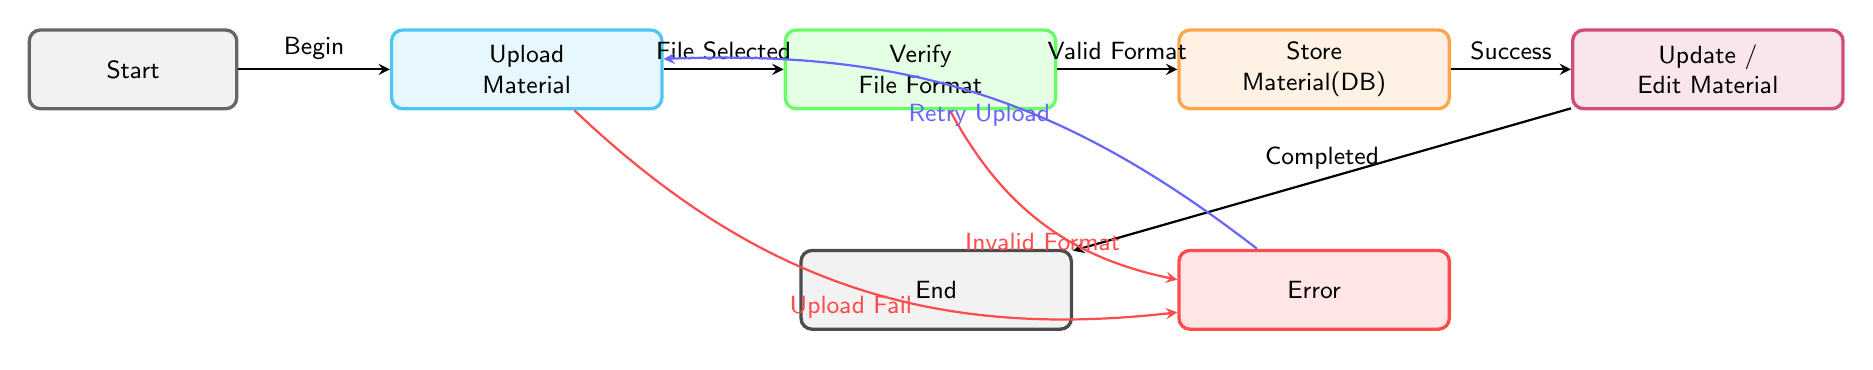
\begin{tikzpicture}[->, >=stealth, node distance=5cm,
			every node/.style={font=\sffamily\small},
			state/.style={rectangle, rounded corners, draw=blue!60, very thick,
				text width=3.2cm, align=center, fill=blue!5, minimum height=1cm}]
			
			% States
			\node[state, fill=gray!10, draw=black!60, text width=2.4cm] (start) {Start};
			\node[state, right of=start, fill=cyan!10, draw=cyan!70] (upload) {Upload\\Material};
			\node[state, right of=upload, fill=green!10, draw=green!60] (verify) {Verify\\File Format};
			\node[state, right of=verify, fill=orange!10, draw=orange!70] (store) {Store\\Material(DB)};
			\node[state, right of=store, fill=purple!10, draw=purple!70] (update) {Update /\\Edit Material};
			\node[state, below of=store, fill=red!10, draw=red!70, node distance=2.8cm] (error) {Error};
			\node[state, left of=error, fill=gray!10, draw=black!70, node distance=4.8cm] (end) {End};
			
			% Transitions
			\path (start) edge[thick] node[above]{Begin} (upload)
			(upload) edge[thick] node[above]{File Selected} (verify)
			(verify) edge[thick] node[above]{Valid Format} (store)
			(store) edge[thick] node[above]{Success} (update)
			(update) edge[thick] node[above]{Completed} (end)
			(verify) edge[bend right=25, thick, red!70] node[below]{Invalid Format} (error)
			(upload) edge[bend right=25, thick, red!70] node[below]{Upload Fail} (error)
			(error) edge[bend right=20, thick, blue!60] node[below]{Retry Upload} (upload);
			
		\end{tikzpicture}
	}
\end{center}

\newpage

\subsection{Class Diagram: Paper Generator Web Application}

The following class diagram represents the structure of the main classes in the system, their attributes, operations, and relationships.

\begin{center}
	\begin{tikzpicture}[every node/.style={font=\sffamily}, >=stealth, scale=0.95, transform shape]
		
		% Classes (Top Row)
		\umlclass[x=0, y=0, fill=yellow!10, draw=orange!70]{Teacher}{
			- teacherID : int \\
			- name : string \\
			- email : string \\
			- password : string
		}{
			+ login() \\
			+ uploadMaterial() \\
			+ generatePaper() \\
			+ exportPaper()
		}
		
		\umlclass[x=6, y=0, fill=cyan!10, draw=cyan!70]{System}{
			- systemID : int \\
			- name : string
		}{
			+ authenticateUser() \\
			+ manageQuestionBank() \\
			+ processPaperGeneration()
		}
		
		\umlclass[x=12, y=0, fill=green!10, draw=green!70]{QuestionBank}{
			- questionID : int \\
			- questionText : string \\
			- topic : string \\
			- difficulty : string
		}{
			+ addQuestion() \\
			+ editQuestion() \\
			+ deleteQuestion() \\
			+ fetchQuestions()
		}
		
		% Classes (Bottom Row - moved downward)
		\umlclass[x=0, y=-7.5, fill=blue!10, draw=blue!70]{ExportModule}{
			- fileType : string \\
			- exportDate : date
		}{
			+ exportToPDF() \\
			+ exportToWord()
		}
		
		\umlclass[x=6, y=-7.5, fill=orange!10, draw=orange!70]{PaperGenerator}{
			- paperID : int \\
			- paperType : string \\
			- difficulty : string
		}{
			+ selectQuestions() \\
			+ createPaper() \\
			+ previewPaper()
		}
		
		\umlclass[x=12, y=-7.5, fill=purple!10, draw=purple!70]{Database}{
			- dbName : string \\
			- host : string
		}{
			+ saveData() \\
			+ retrieveData() \\
			+ backupDatabase()
		}
		
		% Relationships
		\umluniassoc{Teacher}{System}
		\umluniassoc{System}{QuestionBank}
		\umluniassoc{QuestionBank}{System}
		\umluniassoc{System}{PaperGenerator}
		\umluniassoc{PaperGenerator}{Database}
		\umluniassoc{Database}{PaperGenerator}
		\umluniassoc{PaperGenerator}{ExportModule}
		
	\end{tikzpicture}
\end{center}

\noindent
\textbf{Description:} \\
The Class Diagram above represents the main structural components of the Paper Generator Web Application. The \textbf{Teacher} class interacts with the \textbf{System} to authenticate users and initiate operations such as paper generation and exporting. The \textbf{System} manages the workflow by communicating with the \textbf{QuestionBank} to retrieve questions and coordinating with the \textbf{PaperGenerator} for assembling examination papers. The \textbf{PaperGenerator} further interacts with the \textbf{Database} to store and retrieve data, while the \textbf{ExportModule} handles the final conversion of generated papers into printable formats such as PDF or Word. The relationships shown in the diagram highlight a modular, scalable, and maintainable system design, aligning with standard object-oriented development principles.

\subsection{Class Diagram: Question Bank Management}

The following diagram represents the structure and interaction of components involved in managing the question bank within the system.

\begin{center}
	\begin{tikzpicture}[scale=1, transform shape]
		
		% Classes
		\umlclass[x=0, y=0, fill=yellow!10, draw=orange!70]{Teacher}{
			+teacherID : int\\
			+name : string\\
			+email : string
		}{
			+Login()\\
			+AddQuestion()\\
			+EditQuestion()\\
			+DeleteQuestion()\\
			+SearchQuestion()
		}
		
		\umlclass[x=5, y=0, fill=blue!10, draw=blue!70]{QuestionBank}{
			+bankID : int\\
			+subject : string\\
			+topic : string\\
			+difficulty : string
		}{
			+FetchQuestions()\\
			+UpdateQuestion()\\
			+RemoveQuestion()\\
			+CategorizeQuestion()\\
			+GetQuestionList()
		}
		
		\umlclass[x=10, y=0, fill=green!10, draw=green!60]{Question}{
			+questionID : int\\
			+text : string\\
			+type : string\\
			+difficulty : string
		}{
			+Display()\\
			+Edit()\\
			+Validate()\\
			+AssignMarks()
		}
		
		\umlclass[x=5, y=-8.3, fill=purple!10, draw=purple!70]{Database}{
			+dbName : string\\
			+connection : string
		}{
			+StoreQuestion()\\
			+RetrieveQuestions()\\
			+UpdateRecord()\\
			+DeleteRecord()
		}
		
		% Relationships
		\umluniassoc{Teacher}{QuestionBank}
		\umluniassoc{Question}{QuestionBank}
		\umluniassoc{QuestionBank}{Question}
		\umluniassoc{Database}{QuestionBank}
		\umluniassoc{QuestionBank}{Database}
		
		
	\end{tikzpicture}
\end{center}

\noindent
\textbf{Description:} \\
This class diagram illustrates the interactions within the \textbf{Question Bank Management} module. The \textbf{Teacher} manages questions through the system by adding, editing, deleting, and searching them. These operations are handled by the \textbf{QuestionBank} class, which organizes questions by subject, topic, and difficulty. Each individual \textbf{Question} object contains its specific content and attributes, such as text, type, and marks. The \textbf{Database} class ensures reliable data storage and retrieval, keeping the question records synchronized. This diagram aligns with the behavior defined in the sequence diagram for consistent representation of the system’s logic.


\subsection{Class Diagram: Export Module}

The following diagram illustrates the internal structure of the Export Module, aligned with the operations shown in the sequence diagram.

\begin{center}
	\begin{tikzpicture}[scale=1, transform shape]
		
		% Classes
		\umlclass[x=0, y=0, fill=yellow!10, draw=orange!70]{Teacher}{
			+teacherID : int\\
			+name : string\\
			+email : string
		}{
			+Login()\\
			+SelectCourse()\\
			+RequestExport()\\
			+DownloadFile()
		}
		
		\umlclass[x=5, y=0, fill=blue!10, draw=blue!70]{ExportModule}{
			+exportID : int\\
			+formatType : string\\
			+fileName : string
		}{
			+ReceivePaperData()\\
			+ExportPDF()\\
			+ExportWord()\\
			+SendToTeacher()
		}
		
		\umlclass[x=10, y=0, fill=green!10, draw=green!60]{Paper}{
			+paperID : int\\
			+title : string\\
			+marks : int
		}{
			+GeneratePaper()\\
			+GetPaperData()\\
			+FinalizePaper()
		}
		
		\umlclass[x=5, y=-7, fill=purple!10, draw=purple!70]{Database}{
			+dbName : string\\
			+connection : string
		}{
			+FetchPaperData()\\
			+StoreExportLog()
		}
		
		% Relationships
		\umluniassoc{Teacher}{ExportModule}
		\umluniassoc{ExportModule}{Teacher}
		\umluniassoc{ExportModule}{Paper}
		\umluniassoc{Paper}{ExportModule}
		\umluniassoc{ExportModule}{Database}
		\umluniassoc{Database}{ExportModule}
		
		
	\end{tikzpicture}
\end{center}
\newpage
\noindent
\textbf{Description:} \\
This class diagram represents the structure of the \textbf{Export Module} in relation to the entire paper generation workflow. The \textbf{Teacher} logs in, selects a course, and requests an export of the generated paper. The \textbf{ExportModule} receives paper data, converts it into supported formats (PDF or Word), and sends the exported file to the teacher. The \textbf{Paper} class handles generation and preparation of paper content, while the \textbf{Database} ensures data retrieval and maintains export history. This consistent interaction flow ensures system reliability and aligns with the behavior illustrated in the sequence diagram.


\newpage

\subsection{System Activity Diagram: Paper Generator Application}

The following activity diagram illustrates the main operational flow of the Paper Generator Web Application.

\begin{center}
	\resizebox{0.51\textwidth}{!}{%
		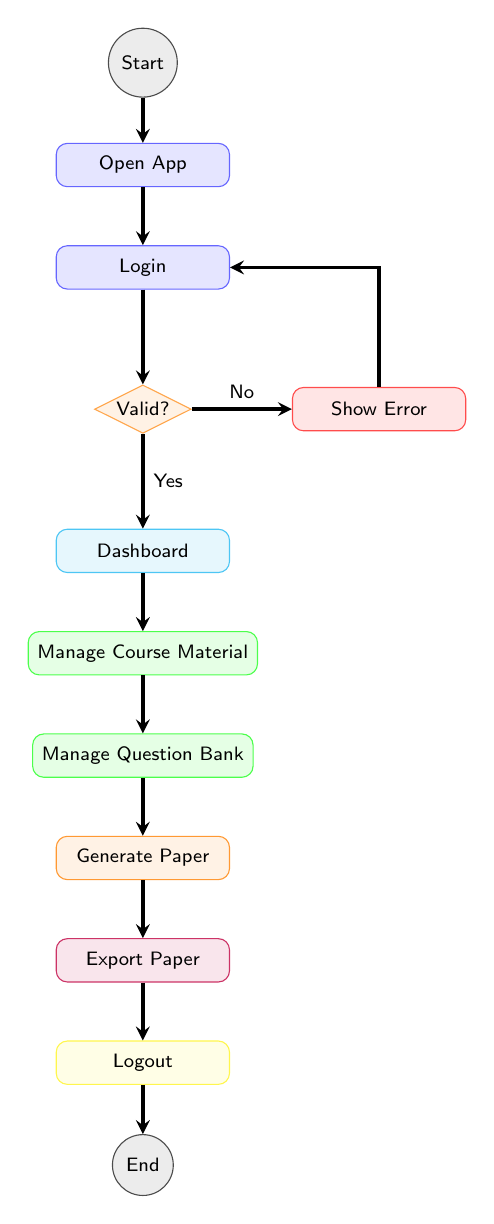
\begin{tikzpicture}[
			>=stealth,
			node distance=1.3cm,
			every node/.style={font=\scriptsize\sffamily}, % Smaller font
			activity/.style={rectangle, rounded corners, draw=blue!60, fill=blue!10,
				minimum width=2.2cm, minimum height=0.55cm, align=center}, % Smaller box
			decision/.style={diamond, draw=orange!70, fill=orange!10,
				aspect=2, inner sep=1pt, align=center},
			startstop/.style={circle, draw=black!70, fill=gray!15,
				minimum size=0.45cm},
			line/.style={->, very thick}
			]
			
			% States
			\node[startstop] (start) {Start};
			
			\node[activity, below of=start] (openapp) {Open App};
			
			\node[activity, below of=openapp] (login) {Login};
			
			\node[decision, below of=login, node distance=1.8cm] (auth) {Valid?};
			
			\node[activity, below of=auth, node distance=1.8cm, fill=cyan!10, draw=cyan!70]
			(dashboard) {Dashboard};
			
			\node[activity, below of=dashboard, fill=green!10, draw=green!70]
			(course) {Manage Course Material};
			
			\node[activity, below of=course, fill=green!10, draw=green!70]
			(qbank) {Manage Question Bank};
			
			\node[activity, below of=qbank, fill=orange!10, draw=orange!80]
			(generate) {Generate Paper};
			
			\node[activity, below of=generate, fill=purple!10, draw=purple!80]
			(export) {Export Paper};
			
			\node[activity, below of=export, fill=yellow!10, draw=yellow!70]
			(logout) {Logout};
			
			\node[startstop, below of=logout] (end) {End};
			
			\node[activity, right of=auth, node distance=3cm, fill=red!10, draw=red!70]
			(error) {Show Error};
			
			% Transitions
			\draw[line] (start) -- (openapp);
			\draw[line] (openapp) -- (login);
			\draw[line] (login) -- (auth);
			
			\draw[line] (auth) -- node[right]{Yes} (dashboard);
			\draw[line] (auth) -- node[above]{No} (error);
			
			\draw[line] (error) |- (login);
			
			\draw[line] (dashboard) -- (course);
			\draw[line] (course) -- (qbank);
			\draw[line] (qbank) -- (generate);
			\draw[line] (generate) -- (export);
			\draw[line] (export) -- (logout);
			\draw[line] (logout) -- (end);
			
		\end{tikzpicture}
	}
\end{center}
\newpage
\noindent\textbf{Description:} \\
This activity diagram illustrates the primary workflow of the Paper Generator Web Application. The process begins when the teacher accesses the system and logs in successfully. After authentication, the user may upload course materials, manage the question bank, and initiate the paper generation process. Once the paper is created, it can be exported for printing or digital distribution. The activity flow ends when the user logs out of the system. In case of failed authentication, the user is redirected back to the login stage. This diagram represents the overall operational behavior of the system in a clear and structured manner.

\newpage

\subsection{Activity Diagram: Paper Generation}

The following activity diagram illustrates the workflow followed by a teacher to generate an exam paper within the system.

\begin{center}
	\resizebox{0.85\textwidth}{!}{
		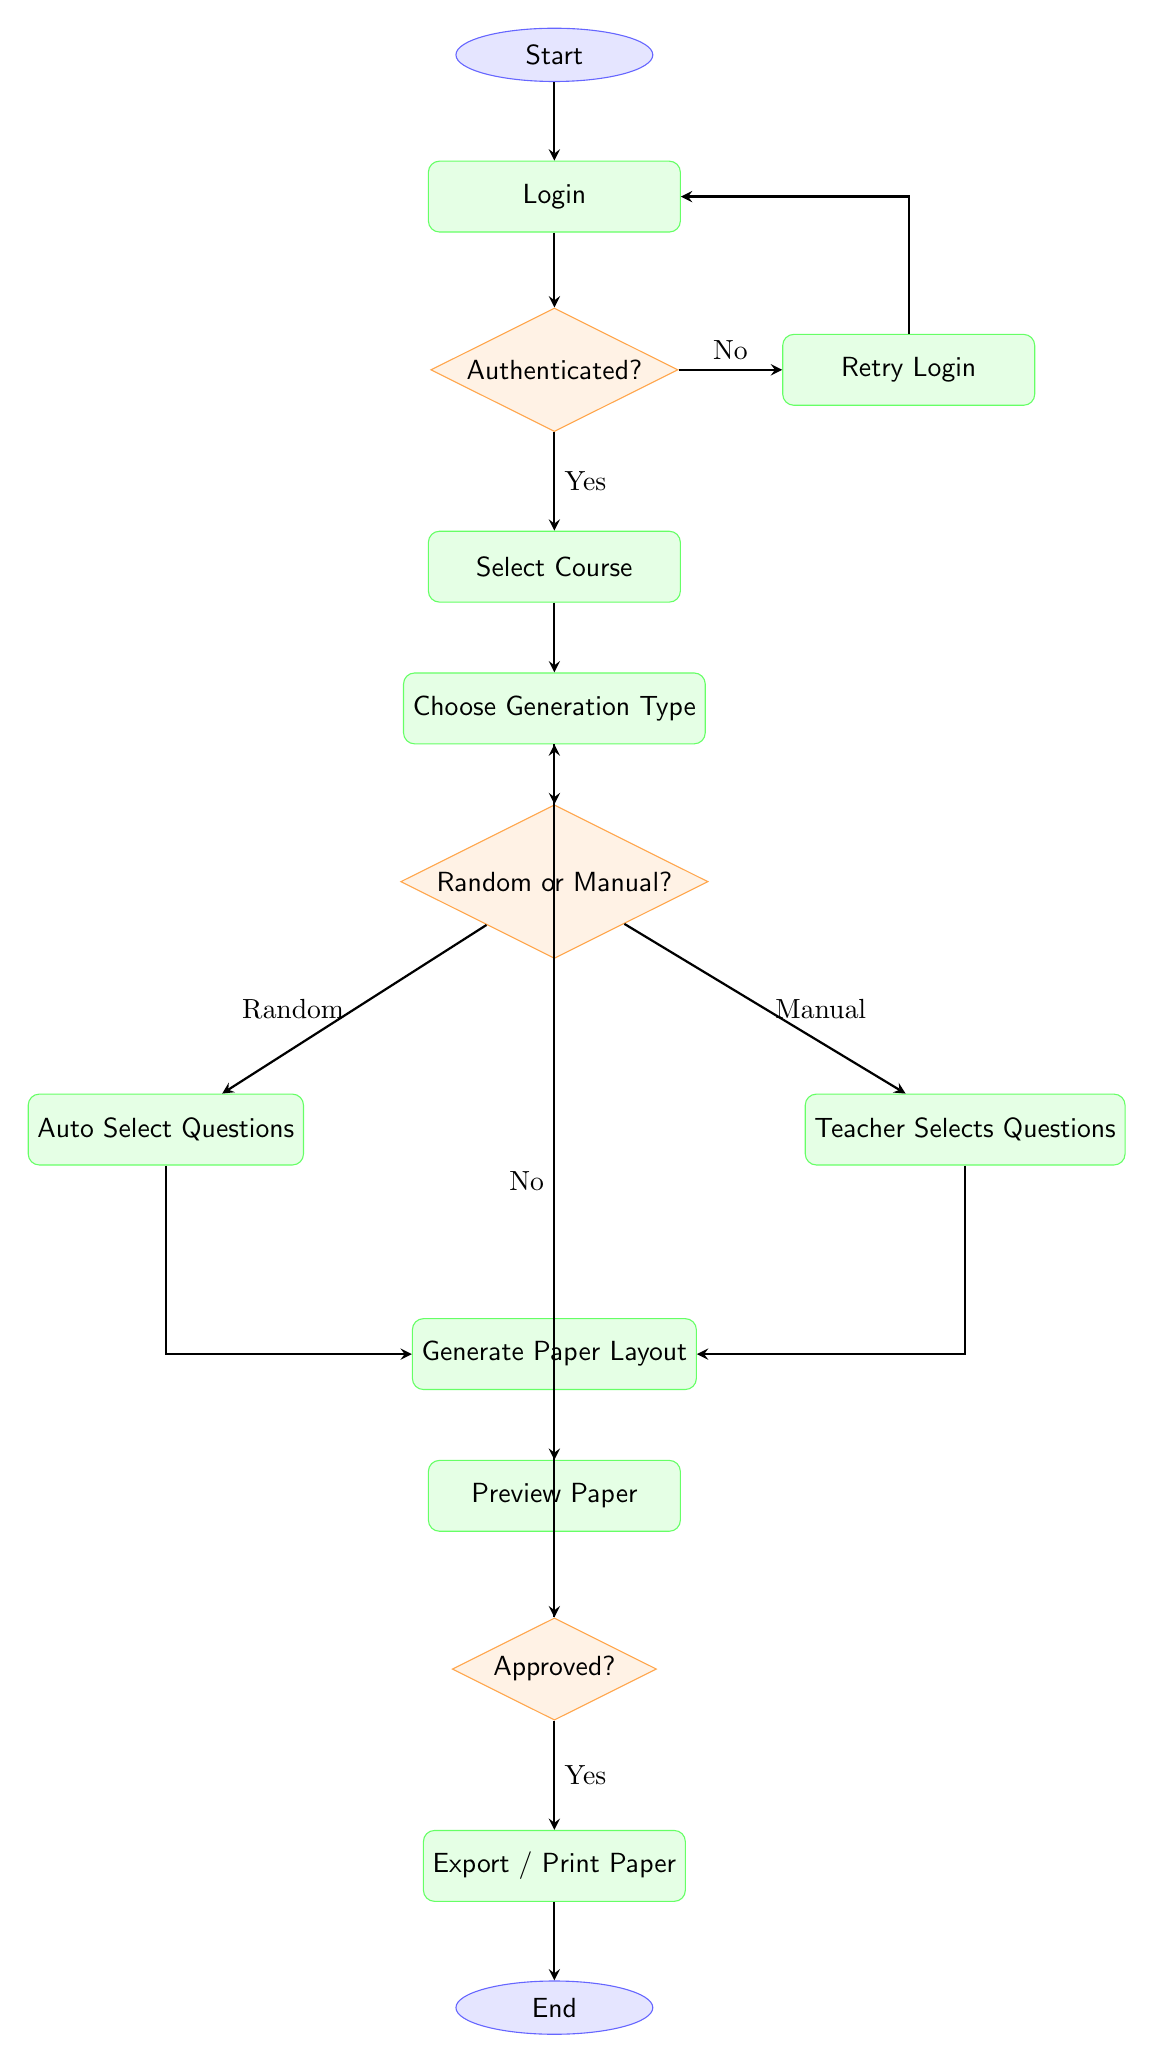
\begin{tikzpicture}[node distance=1.8cm, >=stealth]
			
			% Styles
			\tikzstyle{startstop} = [ellipse, draw=blue!60, fill=blue!10, minimum width=2.5cm, font=\sffamily]
			\tikzstyle{process} = [rectangle, rounded corners, draw=green!60, fill=green!10, minimum width=3.2cm, minimum height=0.9cm, font=\sffamily]
			\tikzstyle{decision} = [diamond, aspect=2, draw=orange!70, fill=orange!10, font=\sffamily, inner sep=2pt]
			\tikzstyle{arrow} = [->, thick]
			
			% Nodes
			\node[startstop] (start) {Start};
			\node[process, below of=start] (login) {Login};
			\node[decision, below of=login, node distance=2.2cm] (auth) {Authenticated?};
			\node[process, below of=auth, node distance=2.5cm] (select) {Select Course};
			\node[process, below of=select] (choose) {Choose Generation Type};
			\node[decision, below of=choose, node distance=2.2cm] (type) {Random or Manual?};
			\node[process, below left=2.2cm and 2.2cm of type] (random) {Auto Select Questions};
			\node[process, below right=2.2cm and 2.2cm of type] (manual) {Teacher Selects Questions};
			\node[process, below of=type, node distance=6cm] (layout) {Generate Paper Layout};
			\node[process, below of=layout] (preview) {Preview Paper};
			\node[decision, below of=preview, node distance=2.2cm] (approve) {Approved?};
			\node[process, below of=approve, node distance=2.5cm] (export) {Export / Print Paper};
			\node[startstop, below of=export] (end) {End};
			
			% Error path
			\node[process, right of=auth, node distance=4.5cm] (retry) {Retry Login};
			
			% Paths
			\draw[arrow] (start) -- (login);
			\draw[arrow] (login) -- (auth);
			\draw[arrow] (auth) -- node[right]{Yes} (select);
			\draw[arrow] (auth) -- node[above]{No} (retry);
			\draw[arrow] (retry) |- (login);
			\draw[arrow] (select) -- (choose);
			\draw[arrow] (choose) -- (type);
			\draw[arrow] (type) -- node[left]{Random} (random);
			\draw[arrow] (type) -- node[right]{Manual} (manual);
			\draw[arrow] (random) |- (layout);
			\draw[arrow] (manual) |- (layout);
			\draw[arrow] (layout) -- (preview);
			\draw[arrow] (preview) -- (approve);
			\draw[arrow] (approve) -- node[right]{Yes} (export);
			\draw[arrow] (approve) -- node[left]{No} (choose);
			\draw[arrow] (export) -- (end);
			
		\end{tikzpicture}
	}
\end{center}


\noindent\textbf{Description:} \\
The above activity diagram illustrates the complete workflow followed by a teacher to generate an examination paper using the Paper Generator Web Application. The process begins when the teacher logs into the system. After successful authentication, the teacher selects the relevant course and chooses whether the paper will be generated manually or randomly.

If random generation is selected, the system automatically retrieves suitable questions from the question bank based on predefined criteria. In manual mode, the teacher individually selects questions. Once selected, the system arranges the questions into a structured exam layout, which is then presented to the teacher for preview.

If the teacher approves the paper, it can be exported or printed for academic use. If not approved, the teacher may revise the selection or regenerate the paper. In case of failed authentication, the system prompts the teacher to retry login. The process concludes once the paper has been successfully exported or printed.


\subsection{ER Diagram}

The  ER diagram illustrates the system entities along with their
attributes, primary keys, and foreign key relationships for the Paper
Generator Web Application.

\begin{center}
\resizebox{0.95\textwidth}{!}{
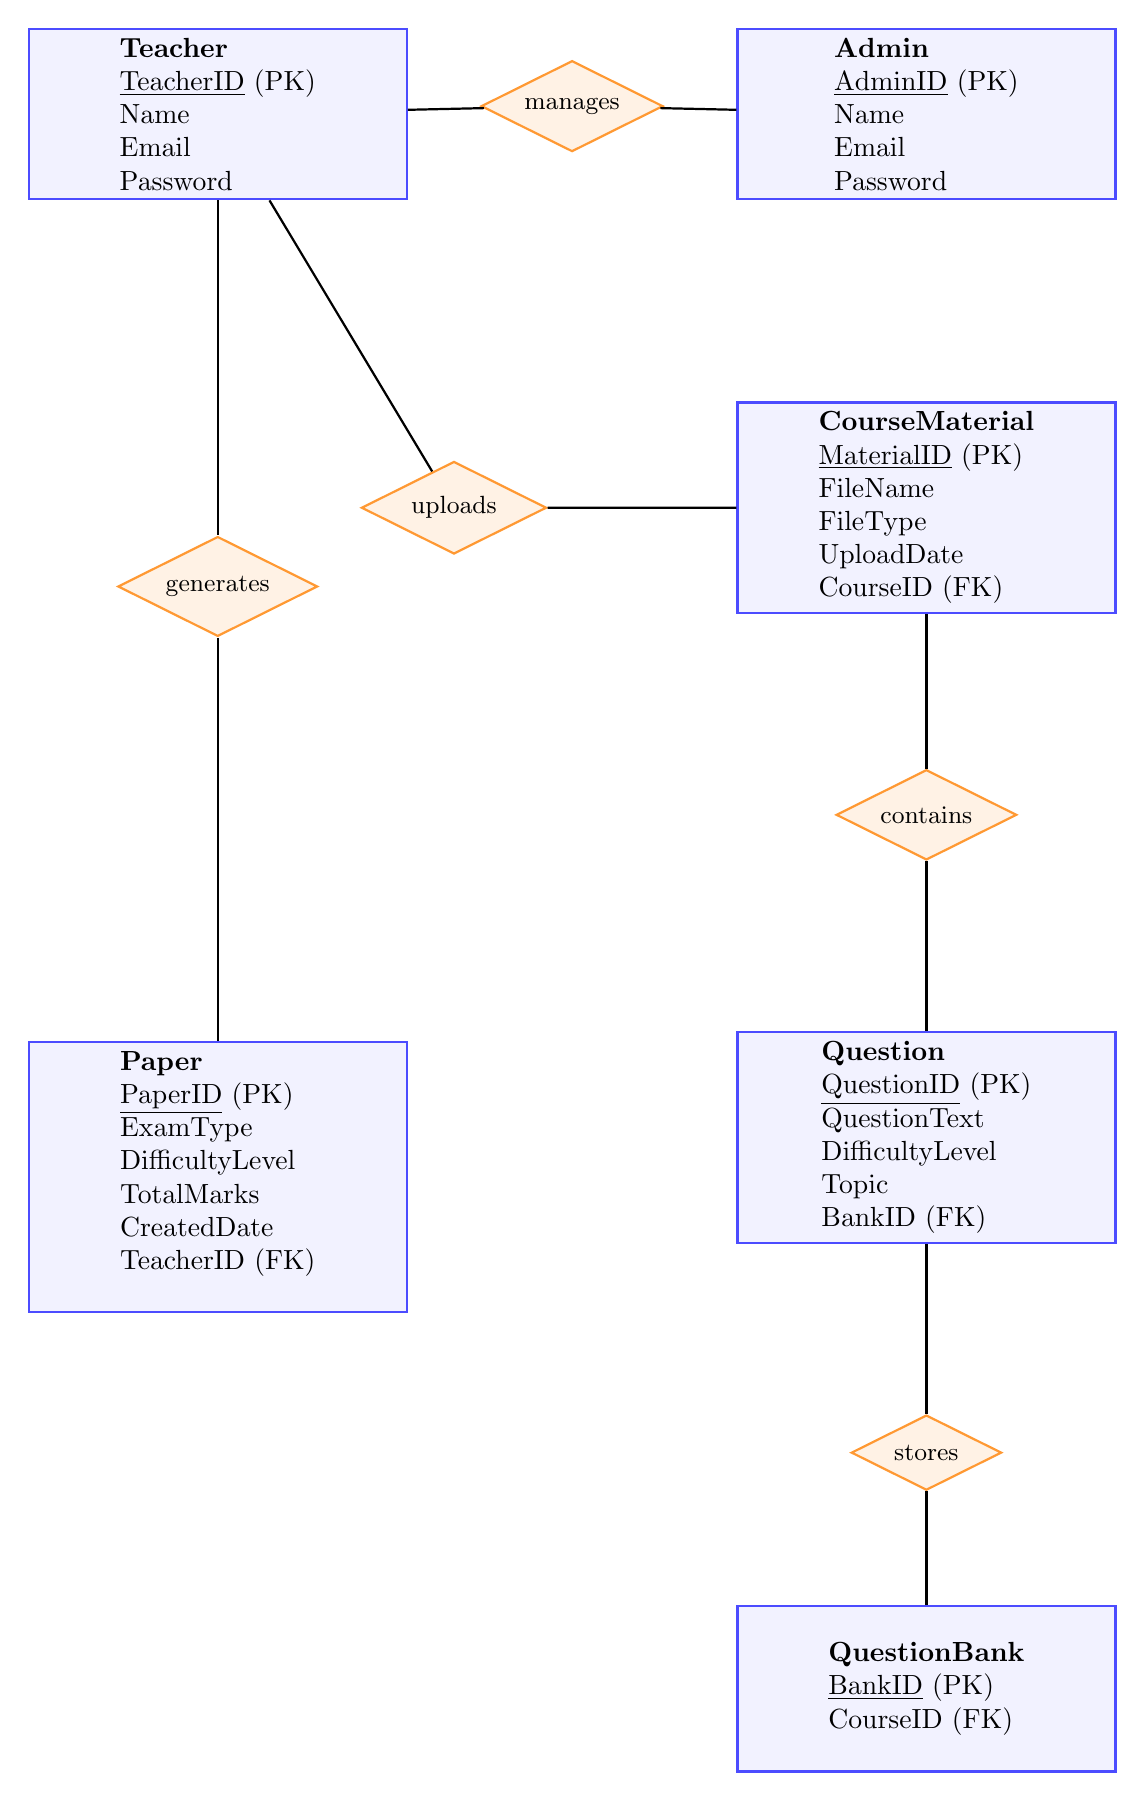
\begin{tikzpicture}[
  entity/.style={
    rectangle,
    draw=blue!70,
    fill=blue!5,
    thick,
    minimum width=4.8cm,
    minimum height=2.1cm,
    align=left
  },
  relation/.style={
    diamond,
    draw=orange!80,
    fill=orange!10,
    thick,
    aspect=2,
    minimum width=1.6cm,
    minimum height=0.7cm,
    font=\small,
    align=center
  },
  line/.style={thick}
]

% ---------- ENTITIES ----------
\node[entity] (Teacher) at (0,0) {
\textbf{Teacher}\\
\underline{TeacherID} (PK)\\
Name\\
Email\\
Password
};

\node[entity] (Admin) at (9,0) {
\textbf{Admin}\\
\underline{AdminID} (PK)\\
Name\\
Email\\
Password
};

% \node[entity] (Course) at (4.5,-3) {
% \textbf{Course}\\
% \underline{CourseID} (PK)\\
% CourseTitle\\
% TeacherID (FK)
% };

\node[entity] (Material) at (9,-5) {
\textbf{CourseMaterial}\\
\underline{MaterialID} (PK)\\
FileName\\
FileType\\
UploadDate\\
CourseID (FK)
};

\node[entity] (QuestionBank) at (9,-20) {
\textbf{QuestionBank}\\
\underline{BankID} (PK)\\
CourseID (FK)
};

\node[entity] (Question) at (9,-13) {
\textbf{Question}\\
\underline{QuestionID} (PK)\\
QuestionText\\
DifficultyLevel\\
Topic\\
BankID (FK)
};

\node[entity] (Paper) at (0,-13.5) {
\textbf{Paper}\\
\underline{PaperID} (PK)\\
ExamType\\
DifficultyLevel\\
TotalMarks\\
CreatedDate\\
TeacherID (FK)\\
};

% ---------- RELATIONSHIPS ----------
% \node[relation] (provides) at (2.2,-1.5) {provides};
\node[relation] (uploads) at (3,-5) {uploads};
\node[relation] (contains) at (9,-8.9) {contains};
\node[relation] (stores) at (9,-17) {stores};
\node[relation] (generates) at (0,-6) {generates};
\node[relation] (manages) at (4.5,0.1) {manages};

% ---------- CONNECTIONS ----------
 
\draw[line] (Teacher) -- (uploads) -- (Material);
% \draw[line] (Course) -- (uploads);
\draw[line] (Material) -- (contains) -- (Question);
\draw[line] (QuestionBank) -- (stores) -- (Question);
\draw[line] (Teacher) -- (generates) -- (Paper);
% \draw[line] (Course) -- (generates);
\draw[line] (Admin) -- (manages) -- (Teacher);

\end{tikzpicture}
}
\end{center}


\subsection{Context Diagram}

The context diagram shows the Paper Generator Web Application as a single
system and illustrates its interaction with external entities.

\begin{center}
\resizebox{0.9\textwidth}{!}{
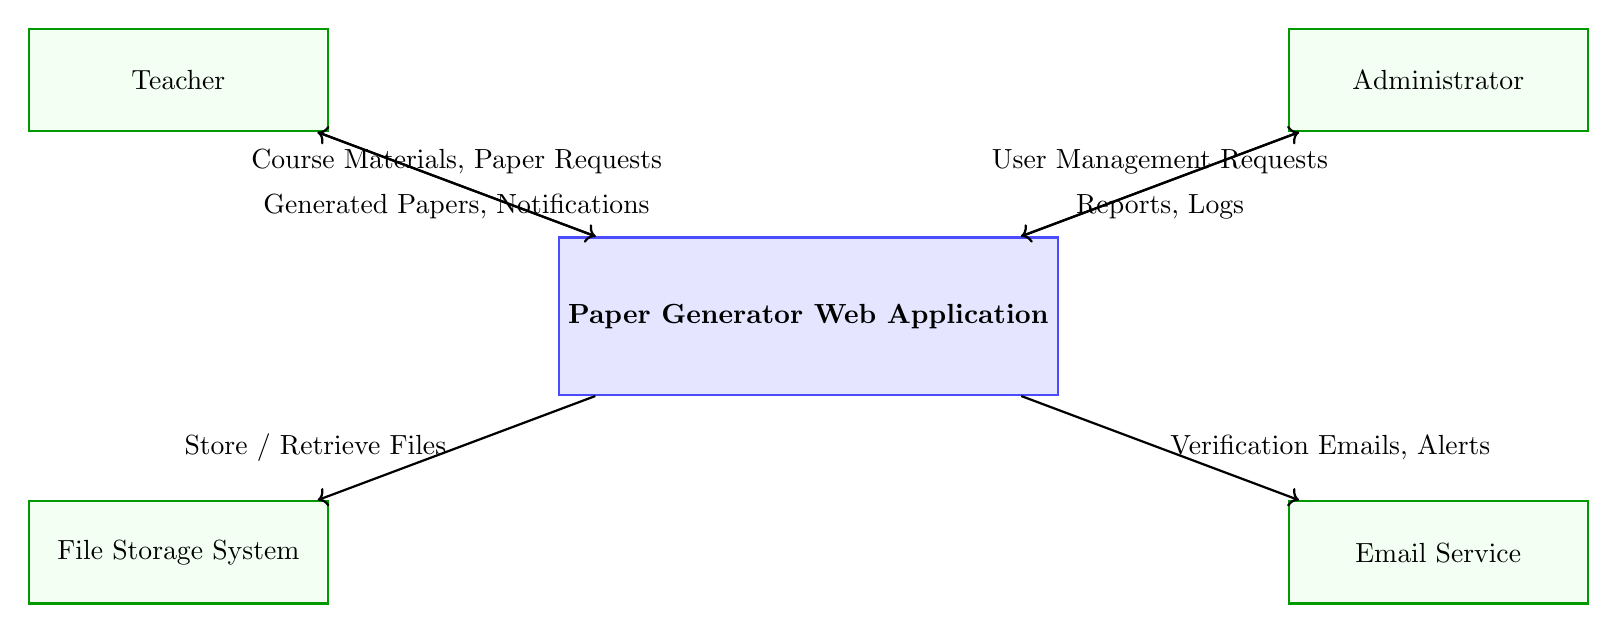
\begin{tikzpicture}[
  process/.style={
    rectangle,
    draw=blue!70,
    fill=blue!10,
    thick,
    minimum width=6cm,
    minimum height=2cm,
    align=center
  },
  external/.style={
    rectangle,
    draw=green!60!black,
    fill=green!5,
    thick,
    minimum width=3.8cm,
    minimum height=1.3cm,
    align=center
  },
  flow/.style={thick, ->}
]

% ---------- Central System ----------
\node[process] (System) at (0,0)
{\textbf{Paper Generator Web Application}};

% ---------- External Entities ----------
\node[external] (Teacher) at (-8,3) {Teacher};
\node[external] (Admin) at (8,3) {Administrator};
\node[external] (Storage) at (-8,-3) {File Storage System};
\node[external] (Email) at (8,-3) {Email Service};

% ---------- Data Flows ----------
\draw[flow] (Teacher) -- node[above] {Course Materials, Paper Requests} (System);
\draw[flow] (System) -- node[below] {Generated Papers, Notifications} (Teacher);

\draw[flow] (Admin) -- node[above] {User Management Requests} (System);
\draw[flow] (System) -- node[below] {Reports, Logs} (Admin);

\draw[flow] (System) -- node[left] {Store / Retrieve Files} (Storage);
\draw[flow] (System) -- node[right] {Verification Emails, Alerts} (Email);

\end{tikzpicture}
}
\end{center}

\subsection{Gantt Chart}

The Gantt chart illustrates the project schedule for the development of the
Paper Generator Web Application, showing the timeline and sequence of major
activities.

\begin{center}
\begin{ganttchart}[
    hgrid,
    vgrid,
    x unit=1.8cm,
    bar/.style={fill=blue!40},
    bar height=0.6
]{1}{6}

% Titles
\gantttitle{Project Timeline (Months)}{6} \\
\gantttitle{Month 1}{1}
\gantttitle{Month 2}{1}
\gantttitle{Month 3}{1}
\gantttitle{Month 4}{1}
\gantttitle{Month 5}{1}
\gantttitle{Month 6}{1} \\

% Tasks
\ganttbar{Project Planning}{1}{1} \\

\ganttbar{Requirement Analysis}{1}{2} \\

\ganttbar{System Design}{2}{3} \\
\ganttbar{ER Diagram}{2}{3} \\

\ganttbar{Database Design}{3}{3} \\

\ganttbar{Implementation}{3}{5} \\

\ganttbar{Testing \& Validation}{4}{5} \\

\ganttbar{Documentation}{5}{6} \\

\ganttbar{Review \& Submission}{6}{6}

\end{ganttchart}
\end{center}

\section{Test case:}

\subsection{Test Case 1: Generate Paper with Valid Inputs}

\begin{table}[H]
\centering
\renewcommand{\arraystretch}{1.1}
\resizebox{\textwidth}{!}{
\begin{tabular}{|p{3.3cm}|p{5.1cm}|p{3.3cm}|p{5.1cm}|}
\hline
\multicolumn{4}{|c|}{\textbf{Test Case Template}} \\ \hline

\textbf{Project Name} & Paper Generator Web Application
& \textbf{Test Designed By} & Talha Niaz\\ \hline

\textbf{Test Case ID} & PG-TC-01
& \textbf{Test Design Date} & 11-01-2026 \\ \hline

\textbf{Test Priority} & High
& \textbf{Test Executed By} & --- \\ \hline

\textbf{Module Name} & Paper Generation
& \textbf{Test Execution Date} & --- \\ \hline

\multicolumn{4}{|l|}{\textbf{Test Title:} Generate paper with valid inputs} \\ \hline

\multicolumn{4}{|l|}{\textbf{Description:}
Verify that the system generates an exam paper successfully when valid exam
parameters are provided by the teacher.} \\ \hline

\multicolumn{4}{|l|}{\textbf{Preconditions:}
Teacher is logged in and sufficient questions exist in the Question Bank.} \\ \hline

\multicolumn{4}{|l|}{\textbf{Dependencies:}
Question Bank Management, Course Material Management} \\ \hline

\multicolumn{4}{|c|}{\textbf{Test Steps}} \\ \hline

\textbf{Step} & \textbf{Test Steps} & \textbf{Test Data} & \textbf{Expected Result} \\ \hline

1 & Select Paper Generation option & --- &
Paper generation interface is displayed \\ \hline

2 & Enter exam type & Midterm &
System accepts exam type \\ \hline

3 & Select subject & Database Systems &
Subject is selected successfully \\ \hline

4 & Choose difficulty level & Moderate &
Difficulty level is accepted \\ \hline

5 & Click Generate Paper & --- &
Draft paper is generated successfully \\ \hline

\multicolumn{4}{|l|}{\textbf{Actual Result:} Draft paper generated successfully} \\ \hline
\multicolumn{4}{|l|}{\textbf{Status:} Pass} \\ \hline
\multicolumn{4}{|l|}{\textbf{Notes:} ---} \\ \hline

\multicolumn{4}{|l|}{\textbf{Postconditions:}
Generated paper is available for review and export.} \\ \hline

\end{tabular}
}
\end{table}

\subsection{Test Case 2: Generate Paper with Insufficient Questions}

\begin{table}[H]
\centering
\renewcommand{\arraystretch}{1.1}
\resizebox{\textwidth}{!}{
\begin{tabular}{|p{3.3cm}|p{5.1cm}|p{3.3cm}|p{5.1cm}|}
\hline
\multicolumn{4}{|c|}{\textbf{Test Case Template}} \\ \hline

\textbf{Project Name} & Paper Generator Web Application
& \textbf{Test Designed By} & Talha Niaz \\ \hline

\textbf{Test Case ID} & PG-TC-02
& \textbf{Test Design Date} & 11-01-2026 \\ \hline

\textbf{Test Priority} & High
& \textbf{Test Executed By} & --- \\ \hline

\textbf{Module Name} & Paper Generation
& \textbf{Test Execution Date} & --- \\ \hline

\multicolumn{4}{|l|}{\textbf{Test Title:} Generate paper with insufficient questions} \\ \hline

\multicolumn{4}{|l|}{\textbf{Description:}
Verify that the system displays an alert when there are not enough questions
available to generate the selected exam paper.} \\ \hline

\multicolumn{4}{|l|}{\textbf{Preconditions:}
Teacher is logged in and the Question Bank contains insufficient questions
for the selected parameters.} \\ \hline

\multicolumn{4}{|l|}{\textbf{Dependencies:}
Question Bank Management, Course Material Management} \\ \hline

\multicolumn{4}{|c|}{\textbf{Test Steps}} \\ \hline

\textbf{Step} & \textbf{Test Steps} & \textbf{Test Data} & \textbf{Expected Result} \\ \hline

1 & Select Paper Generation option & --- &
Paper generation interface is displayed \\ \hline

2 & Enter exam details & Final Exam, Hard &
System accepts input parameters \\ \hline

3 & Click Generate Paper & --- &
System checks question availability \\ \hline

4 & Insufficient questions detected & --- &
System displays warning message \\ \hline

\multicolumn{4}{|l|}{\textbf{Actual Result:}
System displays alert indicating insufficient questions.} \\ \hline

\multicolumn{4}{|l|}{\textbf{Status:} Pass} \\ \hline
\multicolumn{4}{|l|}{\textbf{Notes:}
Teacher is prompted to add more questions or upload course material.} \\ \hline

\multicolumn{4}{|l|}{\textbf{Postconditions:}
No paper is generated until sufficient questions are available.} \\ \hline

\end{tabular}
}
\end{table}

\subsection{Test Case 3: Manage Question Bank}

\begin{table}[H]
\centering
\renewcommand{\arraystretch}{1.1}
\resizebox{\textwidth}{!}{
\begin{tabular}{|p{3.3cm}|p{5.1cm}|p{3.3cm}|p{5.1cm}|}
\hline
\multicolumn{4}{|c|}{\textbf{Test Case Template}} \\ \hline

\textbf{Project Name} & Paper Generator Web Application
& \textbf{Test Designed By} & Talha Niaz \\ \hline

\textbf{Test Case ID} & PG-TC-03
& \textbf{Test Design Date} & 12-01-2026 \\ \hline

\textbf{Test Priority} & High
& \textbf{Test Executed By} & --- \\ \hline

\textbf{Module Name} & Question Bank Management
& \textbf{Test Execution Date} & --- \\ \hline

\multicolumn{4}{|l|}{\textbf{Test Title:} Manage Question Bank operations} \\ \hline

\multicolumn{4}{|l|}{\textbf{Description:}
Verify that the system allows the Teacher to add, edit, delete, categorize,
and retrieve questions successfully in the Question Bank.} \\ \hline

\multicolumn{4}{|l|}{\textbf{Preconditions:}
Teacher is logged in and has permission to manage the Question Bank.} \\ \hline

\multicolumn{4}{|l|}{\textbf{Dependencies:}
User Authentication, Course Material Management} \\ \hline

\multicolumn{4}{|c|}{\textbf{Test Steps}} \\ \hline

\textbf{Step} & \textbf{Test Steps} & \textbf{Test Data} & \textbf{Expected Result} \\ \hline

1 & Open Question Bank Management module & --- &
Question Bank interface is displayed \\ \hline

2 & Add a new question & MCQ, Easy, Software Engineering &
Question is saved successfully \\ \hline

3 & Edit existing question & Update question text &
Question is updated in the system \\ \hline

4 & Search and filter questions & Keyword, Difficulty &
Relevant questions are displayed \\ \hline

5 & Delete a question & Selected question &
System removes the question after confirmation \\ \hline

\multicolumn{4}{|l|}{\textbf{Actual Result:}
System successfully manages Question Bank operations.} \\ \hline

\multicolumn{4}{|l|}{\textbf{Status:} Pass} \\ \hline

\multicolumn{4}{|l|}{\textbf{Notes:}
System prevents duplication and confirms deletion of linked questions.} \\ \hline

\multicolumn{4}{|l|}{\textbf{Postconditions:}
Question Bank is updated with accurate and categorized questions.} \\ \hline

\end{tabular}
}
\end{table}

\end{document}